All data provided by the challenge- and the opendata.cern-dataset \cite{higgsData} was created by the official ATLAS full detector simulator in a two-part-process. The simulator first reproduces proton-proton collisions, called \emph{events}. Then it tracks these via a virtual model of the ATLAS-detector, the resulting data emulates the statistical properties of the real events. By this procedure it is possible to exactly know if an event is a searched \emph{signal}, or \emph{background}. Signal-events are generated by previously mentioned \emph{tau tau decay of the Higgs Boson} ($\mathrm{H}\rightarrow\tau\tau $). Background-events originate from three known processes\footnote{These processes are decay of Z bosons, W bosons and pairs of top quarks. There are more processes known that resemble ($\mathrm{H}\rightarrow\tau\tau $), for simplicity only these three are used as background for this challenge \cite{higgsPaper}.} which produce radiation similar to the signal \cite{higgsPaper}. The feature \texttt{Label} expresses the true class of an event, "$s$" for signals and "$b$" for background.

Every event has a feature \texttt{Weight}, a product of the simulation. The weights correspond to an estimation of the number of expected events of this class in a \emph{region} during a fixed time interval\cite{higgsPaper}.

Assuming, a group of 100 events of both classes "$s$" and "$b$" originate from the same region $A$ and we expect 90\% events of them can be considered as background and 10\% as signal. For another region $B$, we expect a 50/50 distribution. The weights of the events for each region relates directly to our expected probability of this class of event in this specific region. Signal originating from region $A$ are weighted lighter as signal events from region $B$.

This results in a so-called \emph{importance weighting} and causes the weight-mean of signal-events to be considerably smaller than background-weights. We will see, that the challenge evaluation utilizes this to punish incorrectly classifying background as signal.

The features \texttt{Weight} and \texttt{Label} were originally only provided in the training-dataset. The data used in this thesis is expanded by complete \texttt{Weight}-, \texttt{Label}-features and the Kaggle-specific features \texttt{KaggleSet} and \texttt{KaggleWeight}. The last one is a normalization of \texttt{Weight} for the total number of signal- or background-events with the same \texttt{KaggleSet} feature.
This information enables us to recreate the original datasets using the opendata.cern-dataset.

The physical features are separated in two types. Features containing so-called primitive data, properties of events explicitly measured by the simulated ATLAS detector, use the prefix "\texttt{PRI\_}" in their names. The second type is called derived data, which are features that have been computed from primitive features. Their labels use the prefix "\texttt{DER\_}". Tab. \ref{tab:data} is a complete vector retrieved from \cite{higgsData}

\begin{table}
\begin{center}
	\begin{tabular}{|l|r|}
		\hline
		Feature name & Feature value \\
		\hline
		\texttt{EventId} & 100000 \\
		\hline
		\texttt{DER\_mass\_MMC} & 138.47 \\
		\hline
		\texttt{DER\_mass\_transverse\_met\_lep} & 51.655 \\
		\hline
		\texttt{DER\_mass\_vis} & 97.827 \\
		\hline
		\texttt{DER\_pt\_h} & 27.98 \\
		\hline
		\texttt{DER\_deltaeta\_jet\_jet} & 0.91 \\
		\hline
		\texttt{DER\_mass\_jet\_jet} & 124.711 \\
		\hline
		\texttt{DER\_prodeta\_jet\_jet} & 2.666 \\
		\hline
		\texttt{DER\_deltar\_tau\_lep} & 3.064 \\
		\hline
		\texttt{DER\_pt\_tot} & 41.928 \\
		\hline
		\texttt{DER\_sum\_pt} & 197.76 \\
		\hline
		\texttt{DER\_pt\_ratio\_lep\_tau} & 1.582 \\
		\hline
		\texttt{DER\_met\_phi\_centrality} & 1.396 \\
		\hline
		\texttt{DER\_lep\_eta\_centrality} & 0.2 \\
		\hline
		\texttt{PRI\_tau\_pt} & 32.638 \\
		\hline
		\texttt{PRI\_tau\_eta} & 1.017 \\
		\hline
		\texttt{PRI\_tau\_phi} & 0.381 \\
		\hline
		\texttt{PRI\_lep\_pt} & 51.626 \\
		\hline
		\texttt{PRI\_lep\_eta} & 2.273 \\
		\hline
		\texttt{PRI\_lep\_phi} & -2.414 \\
		\hline
		\texttt{PRI\_met} & 16.824 \\
		\hline
		\texttt{PRI\_met\_phi} & -0.277 \\
		\hline
		\texttt{PRI\_met\_sumet} & 258.733 \\
		\hline
		\texttt{PRI\_jet\_num} & 2 \\
		\hline
		\texttt{PRI\_jet\_leading\_pt} & 67.435 \\
		\hline
		\texttt{PRI\_jet\_leading\_eta} & 2.15 \\
		\hline
		\texttt{PRI\_jet\_leading\_phi} & 0.444 \\
		\hline
		\texttt{PRI\_jet\_subleading\_pt} & 46.062 \\
		\hline
		\texttt{PRI\_jet\_subleading\_eta} & 1.24 \\
		\hline
		\texttt{PRI\_jet\_subleading\_phi} & -2.475 \\
		\hline
		\texttt{PRI\_jet\_all\_pt} & 113.497 \\
		\hline
		\texttt{Weight} & 0.00081448039868 \\
		\hline
		\texttt{Label} & s \\
		\hline
		\texttt{KaggleSet} & t \\
		\hline
		\texttt{KaggleWeight} & 0.00265331133733 \\
		\hline	
	\end{tabular}
\end{center}
\caption{Event 100000 provided by opendata.cern data\cite{higgsData}}
\label{tab:data}
\end{table}

One might expect decent physics-knowledge as key in succeeding in the challenge. However, the top-participants did not use a lot domain-knowledge for feature- or method-selection. One goal of the challenges organization was to set a task for data scientists without any physics-background \cite{higgsPaper}.

\subsubsection{Data visualization}
In an first attempt to gain information about our data we use basic methods of data analysis.
To evaluate single features for classification it is common to plot a histogram of the class-labels, in our case "$s$" and "$b$", distribution. A useful way to learn about relations between features is to create \emph{scatter plots} of all two-features-combinations.
Using these visualizations, we can identify features with good properties for our task.

More details about specific features of the dataset can be found in Appendix \ref{app:data}.

\begin{figure}
\centering
\begin{minipage}{.5\textwidth}
  \centering
  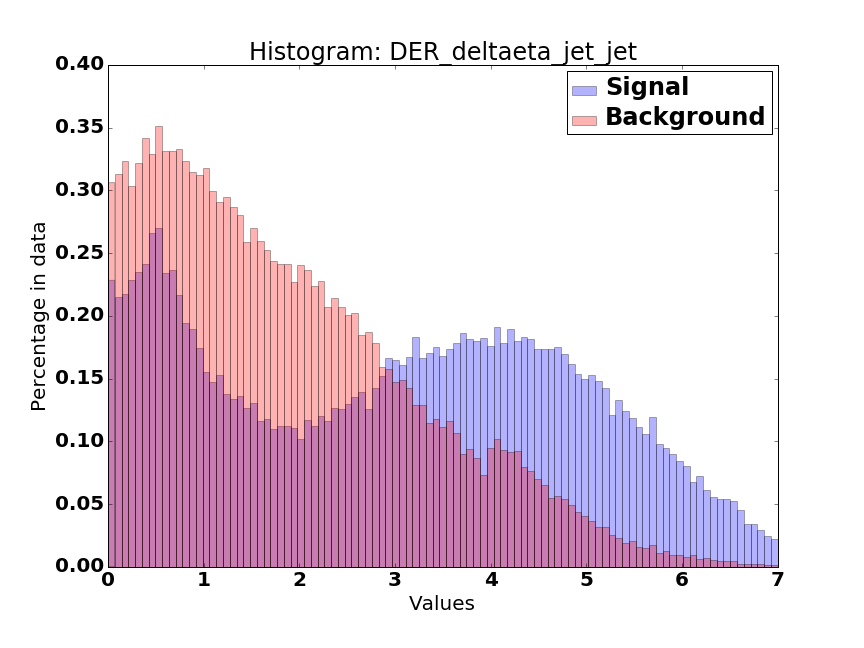
\includegraphics[width=\linewidth]{images/hist_DER_deltaeta_jet_jet}
  \captionof{figure}{\\ Histogram of \emph{DER\_deltaeta\_jet\_jet}}
  \label{fig:hist1}
\end{minipage}%
\begin{minipage}{.5\textwidth}
  \centering
  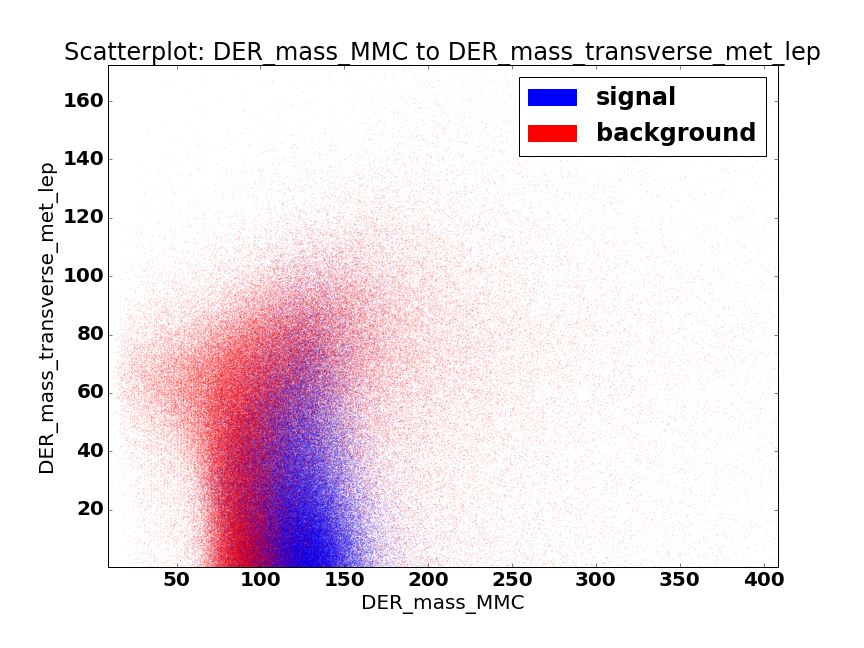
\includegraphics[width=\linewidth]{images/scat_DER_mass_MMCtoDER_mass_transverse_met_lep}
  \captionof{figure}{Scatter plot of \emph{DER\_mass\_MMC} to \emph{DER\_mass\_transverse\_met\_lep}}
  \label{fig:scat1}
\end{minipage}
\end{figure}